	\chapter{Building Blocks of Neural Networks}

	\section{Local Optimum and Saddle Points}
Non-convex functions have local minimums in addition to the global minimum (see \figurename~\ref{fig:complicatedlossfunction}).
 	\begin{figure}[h]
		\centering
		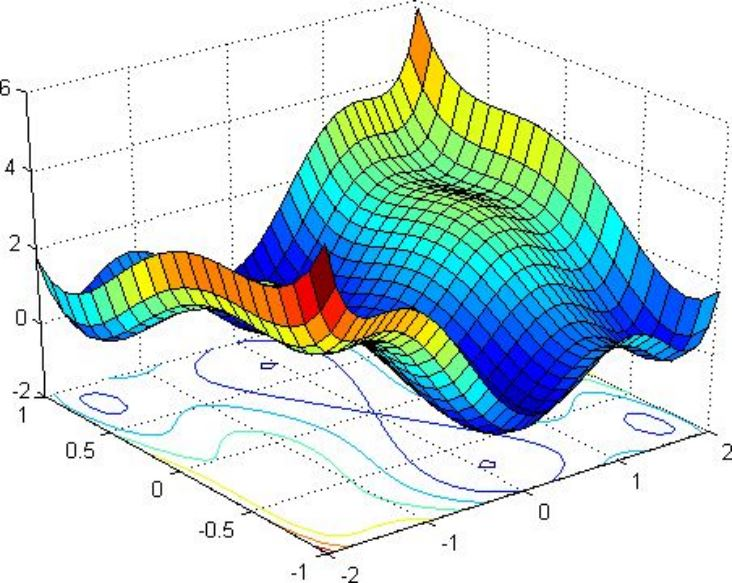
\includegraphics[height=2.0in]{complicatedlossfunction}
		\caption{.}
		\label{fig:complicatedlossfunction}
	\end{figure}

Saddle points, Hessian and long local furrows.  In multiple dimensions:
	\begin{bulletedlist}
		\item Some weights may have reached a local minima while others have not (see \figurename~\ref{fig:saddlepoint}).
		\item Some weights may have almost zero gradient.
		\item This all is characterized by a second derivative matrix called the Hessian, which is difficult to compute and invert.
		\item Different techniques try to approximate Hessian computation and inversion.
		\item Usually, they treat each weight independently and set learning rates for each differently.
		\item Examples: RMSprop, ADAM, Nesterov momentum.
	\end{bulletedlist}
 	\begin{figure}[h]
		\centering
		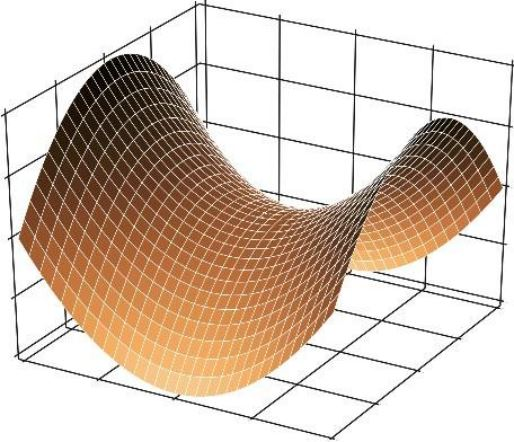
\includegraphics[height=2.0in]{saddlepoint}
		\caption{.}
		\label{fig:saddlepoint}
	\end{figure}


	\section{Other variants of Gradient Descent}
What is the need for advanced optimization?
	\begin{bulletedlist}
		\item Slow conversion rate.
		\item Gradient gets stuck in the local optima
	\end{bulletedlist}

Gradient descent optimization algorithms:
	\begin{bulletedlist}
		\item Gradient descent
		\item Stochastic Gradient Descent
		\item Mini Batch Gradient descent
		\item Gradient descent Momentum
		\item RMS prop
		\item Adam
	\end{bulletedlist}

In this course, we will be discussing RMSprop and Adam.

	\section{Stochastic Gradient Descent with Momentum}

	\begin{bulletedlist}
		\item Stochastic Gradient Descent is an optimization algorithm used in Machine Learning.
		\item During the training period to find the derivative loss function random data point is selected instead of whole data for each iteration.  For Example: A data set consists of 1000 data points and to calculate the derivative loss function it will be considering only one data point at a time.
		\item In SGD convergence to global minima happens very slowly as it will take a single record in each iteration during forward and backward propagation.
	\end{bulletedlist}
see \figurename~\ref{fig:stochasticgradientdescent}
 	\begin{figure}[h]
		\centering
		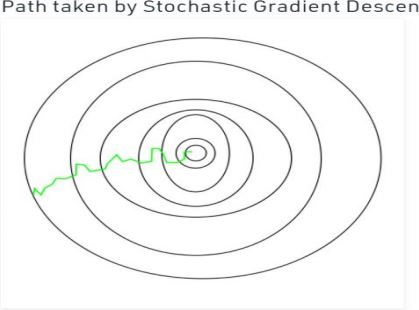
\includegraphics[height=2.0in]{stochasticgradientdescent}
		\caption{.}
		\label{fig:stochasticgradientdescent}
	\end{figure}

	\begin{bulletedlist}
		\item To overcome the noisy data produced by the Mini batch Gradient descent there is another variant of Gradient Descent called Gradient descent with momentum which will smoothen the noisy data.
		\item Gradient Descent with Momentum uses exponentially weighted averages of gradients over the previous iteration to stabilize the convergence (see \figurename~\ref{fig:stochasticgradientdescent}).
	\end{bulletedlist}
 	\begin{figure}[h]
		\centering
		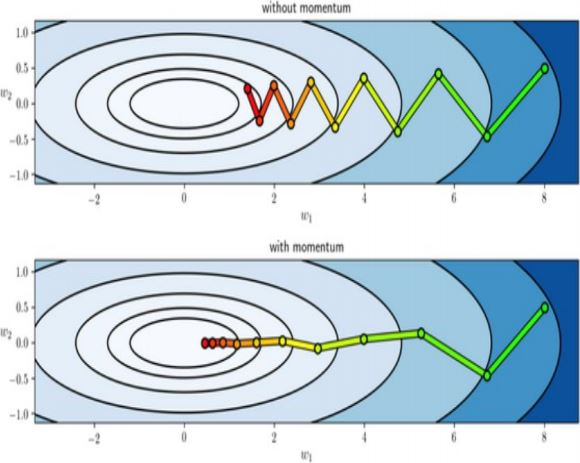
\includegraphics[height=2.0in]{stochasticgradientdescentmomentum}
		\caption{.}
		\label{fig:stochasticgradientdescentmomentum}
	\end{figure}


	\section{RMSprop}

	\begin{bulletedlist}
		\item RMSprop optimization is termed as root mean squared propagation optimization technique.
		\item It is a gradient based optimization technique used in training a neural network.
		\item Gradients of very complex functions like neural networks have a tendency to either vanish or explode as the data propagates through the function.
		\item RMSprop deals with this issue by using a moving average of squared gradients to normalize the gradient.
		\item This balances the step size, decreasing the step for large gradients to avoid exploding and increasing the step for small gradients to avoid vanishing.
		\item RMSprop is preferred over gradient descent because it has a very good convergence speed towards the minima of the cost function.
	\end{bulletedlist}

	\subsection{How it Works}
Please reference \figurename~\ref{fig:rmsprophowitworks} for the following:
	\begin{bulletedlist}
		\item Here Vdw and Vdb are the exponential averages of squares of gradients.
		\item $\beta$ is a hyperparameter and W is the weight term.
		\item dw2 and db2 are the second-order derivative of the cost function with respect to the weight and bias respectively.
		\item $\alpha$ is the learning rate. In RMSprop learning rate is not a hyperparameter.  It is managed by the algorithm itself, instead of being tuned.
		\item $\epsilon$ epsilon is the additive term.  It just ensures that the denominator does not get equal to zero when Vdb or Vdw becomes equal to zero.  Ideally, its value is 10-8.
		\item Ideally, dw is small and db is high. Hence step size of w increases(divided by a smaller number) and that of b decreases(divided by a larger number).  Due to this the convergence in the direction of weight increases in RMSprop.
	\end{bulletedlist}
 	\begin{figure}[h]
		\centering
		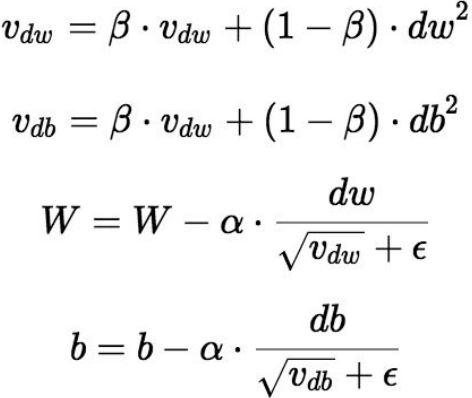
\includegraphics[height=2.0in]{rmsprophowitworks}
		\caption{.}
		\label{fig:rmsprophowitworks}
	\end{figure}


	\section{Weight initialization and its Techniques}
	\section{Regularization}

	\section{Dropout}
	\section{Batch Normalization}
	\section{Types of Neural Networks}
	\section{Hands On Neural Network}